% Options for packages loaded elsewhere
\PassOptionsToPackage{unicode}{hyperref}
\PassOptionsToPackage{hyphens}{url}
%
\documentclass[
]{article}
\usepackage{amsmath,amssymb}
\usepackage{iftex}
\ifPDFTeX
  \usepackage[T1]{fontenc}
  \usepackage[utf8]{inputenc}
  \usepackage{textcomp} % provide euro and other symbols
\else % if luatex or xetex
  \usepackage{unicode-math} % this also loads fontspec
  \defaultfontfeatures{Scale=MatchLowercase}
  \defaultfontfeatures[\rmfamily]{Ligatures=TeX,Scale=1}
\fi
\usepackage{lmodern}
\ifPDFTeX\else
  % xetex/luatex font selection
\fi
% Use upquote if available, for straight quotes in verbatim environments
\IfFileExists{upquote.sty}{\usepackage{upquote}}{}
\IfFileExists{microtype.sty}{% use microtype if available
  \usepackage[]{microtype}
  \UseMicrotypeSet[protrusion]{basicmath} % disable protrusion for tt fonts
}{}
\makeatletter
\@ifundefined{KOMAClassName}{% if non-KOMA class
  \IfFileExists{parskip.sty}{%
    \usepackage{parskip}
  }{% else
    \setlength{\parindent}{0pt}
    \setlength{\parskip}{6pt plus 2pt minus 1pt}}
}{% if KOMA class
  \KOMAoptions{parskip=half}}
\makeatother
\usepackage{xcolor}
\usepackage[margin=1in]{geometry}
\usepackage{color}
\usepackage{fancyvrb}
\newcommand{\VerbBar}{|}
\newcommand{\VERB}{\Verb[commandchars=\\\{\}]}
\DefineVerbatimEnvironment{Highlighting}{Verbatim}{commandchars=\\\{\}}
% Add ',fontsize=\small' for more characters per line
\usepackage{framed}
\definecolor{shadecolor}{RGB}{248,248,248}
\newenvironment{Shaded}{\begin{snugshade}}{\end{snugshade}}
\newcommand{\AlertTok}[1]{\textcolor[rgb]{0.94,0.16,0.16}{#1}}
\newcommand{\AnnotationTok}[1]{\textcolor[rgb]{0.56,0.35,0.01}{\textbf{\textit{#1}}}}
\newcommand{\AttributeTok}[1]{\textcolor[rgb]{0.13,0.29,0.53}{#1}}
\newcommand{\BaseNTok}[1]{\textcolor[rgb]{0.00,0.00,0.81}{#1}}
\newcommand{\BuiltInTok}[1]{#1}
\newcommand{\CharTok}[1]{\textcolor[rgb]{0.31,0.60,0.02}{#1}}
\newcommand{\CommentTok}[1]{\textcolor[rgb]{0.56,0.35,0.01}{\textit{#1}}}
\newcommand{\CommentVarTok}[1]{\textcolor[rgb]{0.56,0.35,0.01}{\textbf{\textit{#1}}}}
\newcommand{\ConstantTok}[1]{\textcolor[rgb]{0.56,0.35,0.01}{#1}}
\newcommand{\ControlFlowTok}[1]{\textcolor[rgb]{0.13,0.29,0.53}{\textbf{#1}}}
\newcommand{\DataTypeTok}[1]{\textcolor[rgb]{0.13,0.29,0.53}{#1}}
\newcommand{\DecValTok}[1]{\textcolor[rgb]{0.00,0.00,0.81}{#1}}
\newcommand{\DocumentationTok}[1]{\textcolor[rgb]{0.56,0.35,0.01}{\textbf{\textit{#1}}}}
\newcommand{\ErrorTok}[1]{\textcolor[rgb]{0.64,0.00,0.00}{\textbf{#1}}}
\newcommand{\ExtensionTok}[1]{#1}
\newcommand{\FloatTok}[1]{\textcolor[rgb]{0.00,0.00,0.81}{#1}}
\newcommand{\FunctionTok}[1]{\textcolor[rgb]{0.13,0.29,0.53}{\textbf{#1}}}
\newcommand{\ImportTok}[1]{#1}
\newcommand{\InformationTok}[1]{\textcolor[rgb]{0.56,0.35,0.01}{\textbf{\textit{#1}}}}
\newcommand{\KeywordTok}[1]{\textcolor[rgb]{0.13,0.29,0.53}{\textbf{#1}}}
\newcommand{\NormalTok}[1]{#1}
\newcommand{\OperatorTok}[1]{\textcolor[rgb]{0.81,0.36,0.00}{\textbf{#1}}}
\newcommand{\OtherTok}[1]{\textcolor[rgb]{0.56,0.35,0.01}{#1}}
\newcommand{\PreprocessorTok}[1]{\textcolor[rgb]{0.56,0.35,0.01}{\textit{#1}}}
\newcommand{\RegionMarkerTok}[1]{#1}
\newcommand{\SpecialCharTok}[1]{\textcolor[rgb]{0.81,0.36,0.00}{\textbf{#1}}}
\newcommand{\SpecialStringTok}[1]{\textcolor[rgb]{0.31,0.60,0.02}{#1}}
\newcommand{\StringTok}[1]{\textcolor[rgb]{0.31,0.60,0.02}{#1}}
\newcommand{\VariableTok}[1]{\textcolor[rgb]{0.00,0.00,0.00}{#1}}
\newcommand{\VerbatimStringTok}[1]{\textcolor[rgb]{0.31,0.60,0.02}{#1}}
\newcommand{\WarningTok}[1]{\textcolor[rgb]{0.56,0.35,0.01}{\textbf{\textit{#1}}}}
\usepackage{graphicx}
\makeatletter
\def\maxwidth{\ifdim\Gin@nat@width>\linewidth\linewidth\else\Gin@nat@width\fi}
\def\maxheight{\ifdim\Gin@nat@height>\textheight\textheight\else\Gin@nat@height\fi}
\makeatother
% Scale images if necessary, so that they will not overflow the page
% margins by default, and it is still possible to overwrite the defaults
% using explicit options in \includegraphics[width, height, ...]{}
\setkeys{Gin}{width=\maxwidth,height=\maxheight,keepaspectratio}
% Set default figure placement to htbp
\makeatletter
\def\fps@figure{htbp}
\makeatother
\setlength{\emergencystretch}{3em} % prevent overfull lines
\providecommand{\tightlist}{%
  \setlength{\itemsep}{0pt}\setlength{\parskip}{0pt}}
\setcounter{secnumdepth}{-\maxdimen} % remove section numbering
\ifLuaTeX
  \usepackage{selnolig}  % disable illegal ligatures
\fi
\IfFileExists{bookmark.sty}{\usepackage{bookmark}}{\usepackage{hyperref}}
\IfFileExists{xurl.sty}{\usepackage{xurl}}{} % add URL line breaks if available
\urlstyle{same}
\hypersetup{
  pdftitle={Activity monitoring analysis},
  pdfauthor={Varenka Rico},
  hidelinks,
  pdfcreator={LaTeX via pandoc}}

\title{Activity monitoring analysis}
\author{Varenka Rico}
\date{2023-11-01}

\begin{document}
\maketitle

\hypertarget{abstract}{%
\subsection{Abstract}\label{abstract}}

The objective of this analysis is determine whether it seems to be a
different walking activity through the day, as well as determine if
activity changes during weekdays and weekends. There have been some data
cleaning process to fill null values with average values. The results
show there are different moments through the day that activity increases
and decreases, and the number of steps during weekdays and weekends do
have some difference.

\hypertarget{analysis-process}{%
\subsection{Analysis process}\label{analysis-process}}

\hypertarget{libraries-required}{%
\subsubsection{Libraries required}\label{libraries-required}}

library(tidyverse)\\
library(lubridate)

\hypertarget{getting-information}{%
\subsubsection{Getting information}\label{getting-information}}

In order to avoid downloading any file into the computer, a temp file is
created. The information was downloaded on November 1st, 2023.

\begin{Shaded}
\begin{Highlighting}[]
\NormalTok{temp }\OtherTok{\textless{}{-}} \FunctionTok{tempfile}\NormalTok{()}
\FunctionTok{download.file}\NormalTok{(}\StringTok{"https://d396qusza40orc.cloudfront.net/repdata\%2Fdata\%2Factivity.zip?raw=TRUE"}\NormalTok{, }
\NormalTok{              temp, }\AttributeTok{mode =} \StringTok{"wb"}\NormalTok{)}
\NormalTok{raw\_data }\OtherTok{\textless{}{-}}\FunctionTok{read.csv}\NormalTok{(}\FunctionTok{unzip}\NormalTok{(temp,}\StringTok{"activity.csv"}\NormalTok{))}
\FunctionTok{unlink}\NormalTok{(temp)}
\end{Highlighting}
\end{Shaded}

\hypertarget{understanding-the-information}{%
\subsubsection{Understanding the
information}\label{understanding-the-information}}

The table has 3 columns:

\textbf{steps:} Number of steps taking in a 5-minute interval (missing
values are coded as NA)\\
\textbf{date:} The date on which the measurement was taken in YYYY-MM-DD
format\\
\textbf{interval:} Identifier for the 5-minute interval in which
measurement was taken

\begin{Shaded}
\begin{Highlighting}[]
\FunctionTok{head}\NormalTok{(raw\_data)}
\end{Highlighting}
\end{Shaded}

\begin{verbatim}
##   steps       date interval
## 1    NA 2012-10-01        0
## 2    NA 2012-10-01        5
## 3    NA 2012-10-01       10
## 4    NA 2012-10-01       15
## 5    NA 2012-10-01       20
## 6    NA 2012-10-01       25
\end{verbatim}

\begin{Shaded}
\begin{Highlighting}[]
\FunctionTok{summary}\NormalTok{(raw\_data)}
\end{Highlighting}
\end{Shaded}

\begin{verbatim}
##      steps            date              interval     
##  Min.   :  0.00   Length:17568       Min.   :   0.0  
##  1st Qu.:  0.00   Class :character   1st Qu.: 588.8  
##  Median :  0.00   Mode  :character   Median :1177.5  
##  Mean   : 37.38                      Mean   :1177.5  
##  3rd Qu.: 12.00                      3rd Qu.:1766.2  
##  Max.   :806.00                      Max.   :2355.0  
##  NA's   :2304
\end{verbatim}

\hypertarget{missing-data---identification}{%
\paragraph{Missing data -
Identification}\label{missing-data---identification}}

There are 2304 NAs in the data. All of them for the days 2012-10-01,
2012-10-08, 2012-11-01, 2012-11-04, 2012-11-09, 2012-11-10, 2012-11-14,
2012-11-30.

To make sure all the days have 288 5-minute periods, it is necessary to
count the number of measurements done each day and plot it.

\begin{Shaded}
\begin{Highlighting}[]
\NormalTok{df\_5min\_periods }\OtherTok{\textless{}{-}} \FunctionTok{aggregate}\NormalTok{(raw\_data}\SpecialCharTok{$}\NormalTok{steps, }\AttributeTok{by =} \FunctionTok{list}\NormalTok{(}\FunctionTok{ymd}\NormalTok{(raw\_data}\SpecialCharTok{$}\NormalTok{date)), }\AttributeTok{FUN =}\NormalTok{ length)}
\NormalTok{df\_5min\_periods }\OtherTok{\textless{}{-}} \FunctionTok{setNames}\NormalTok{(df\_5min\_periods, }\FunctionTok{c}\NormalTok{(}\StringTok{"date"}\NormalTok{, }\StringTok{"num\_periods"}\NormalTok{))}
\end{Highlighting}
\end{Shaded}

\begin{Shaded}
\begin{Highlighting}[]
\FunctionTok{ggplot}\NormalTok{(}\AttributeTok{data =}\NormalTok{ df\_5min\_periods, }\FunctionTok{aes}\NormalTok{(}\AttributeTok{x=}\NormalTok{date, }\AttributeTok{y=}\NormalTok{num\_periods)) }\SpecialCharTok{+}
  \FunctionTok{geom\_bar}\NormalTok{(}\AttributeTok{stat=}\StringTok{"identity"}\NormalTok{) }\SpecialCharTok{+}
  \FunctionTok{labs}\NormalTok{(}\AttributeTok{title =} \StringTok{"Total 5{-}minute periods per day"}\NormalTok{)}
\end{Highlighting}
\end{Shaded}

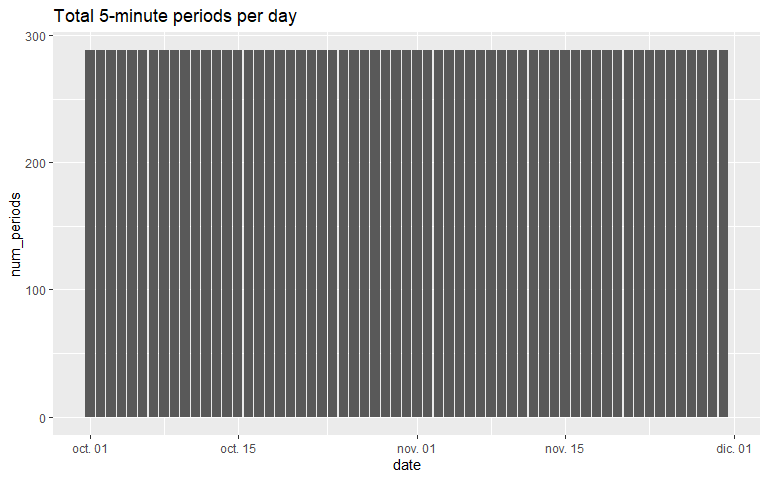
\includegraphics{PA1_template_files/figure-latex/barplot_5min_periods-1.pdf}

\hypertarget{steps-by-day}{%
\subsection{Steps by day}\label{steps-by-day}}

To determine the total number of steps taken each day, it is necessary
to sum the steps in each 5-minute period for each day first.

\begin{Shaded}
\begin{Highlighting}[]
\NormalTok{df\_by\_day }\OtherTok{\textless{}{-}} \FunctionTok{aggregate}\NormalTok{(raw\_data}\SpecialCharTok{$}\NormalTok{steps, }\AttributeTok{by =} \FunctionTok{list}\NormalTok{(}\FunctionTok{ymd}\NormalTok{(raw\_data}\SpecialCharTok{$}\NormalTok{date)), }\AttributeTok{FUN =}\NormalTok{ sum)}
\NormalTok{df\_by\_day }\OtherTok{\textless{}{-}} \FunctionTok{setNames}\NormalTok{(df\_by\_day, }\FunctionTok{c}\NormalTok{(}\StringTok{"date"}\NormalTok{, }\StringTok{"steps"}\NormalTok{))}
\end{Highlighting}
\end{Shaded}

\begin{Shaded}
\begin{Highlighting}[]
\FunctionTok{ggplot}\NormalTok{(}\AttributeTok{data =}\NormalTok{ df\_by\_day, }\FunctionTok{aes}\NormalTok{(}\AttributeTok{x=}\NormalTok{date, }\AttributeTok{y=}\NormalTok{steps)) }\SpecialCharTok{+}
  \FunctionTok{geom\_bar}\NormalTok{(}\AttributeTok{stat=}\StringTok{"identity"}\NormalTok{) }\SpecialCharTok{+}
  \FunctionTok{labs}\NormalTok{(}\AttributeTok{title =} \StringTok{"Total steps by day"}\NormalTok{)}
\end{Highlighting}
\end{Shaded}

\begin{verbatim}
## Warning: Removed 8 rows containing missing values (`position_stack()`).
\end{verbatim}

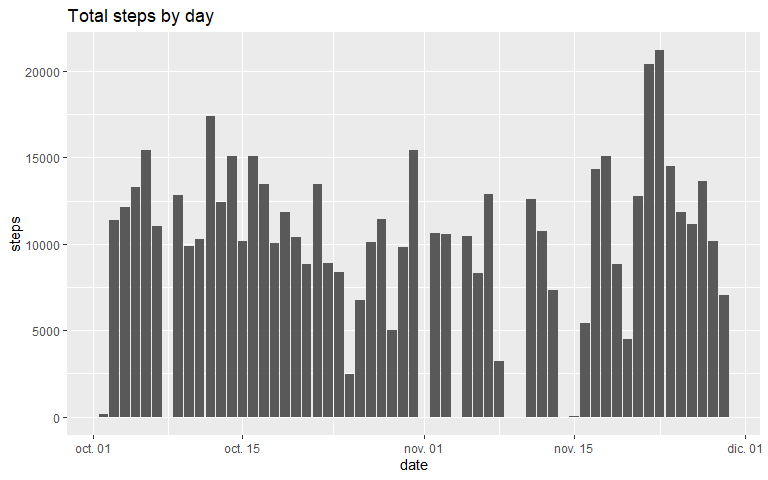
\includegraphics{PA1_template_files/figure-latex/bar_plot-1.pdf}

\begin{Shaded}
\begin{Highlighting}[]
\FunctionTok{ggplot}\NormalTok{(}\AttributeTok{data =}\NormalTok{ df\_by\_day, }\FunctionTok{aes}\NormalTok{(}\AttributeTok{x=}\NormalTok{steps)) }\SpecialCharTok{+}
  \FunctionTok{geom\_histogram}\NormalTok{(}\AttributeTok{bins =} \DecValTok{10}\NormalTok{) }\SpecialCharTok{+}
  \FunctionTok{labs}\NormalTok{(}\AttributeTok{title =} \StringTok{"Histogram of steps{-}by{-}day"}\NormalTok{)}
\end{Highlighting}
\end{Shaded}

\begin{verbatim}
## Warning: Removed 8 rows containing non-finite values (`stat_bin()`).
\end{verbatim}

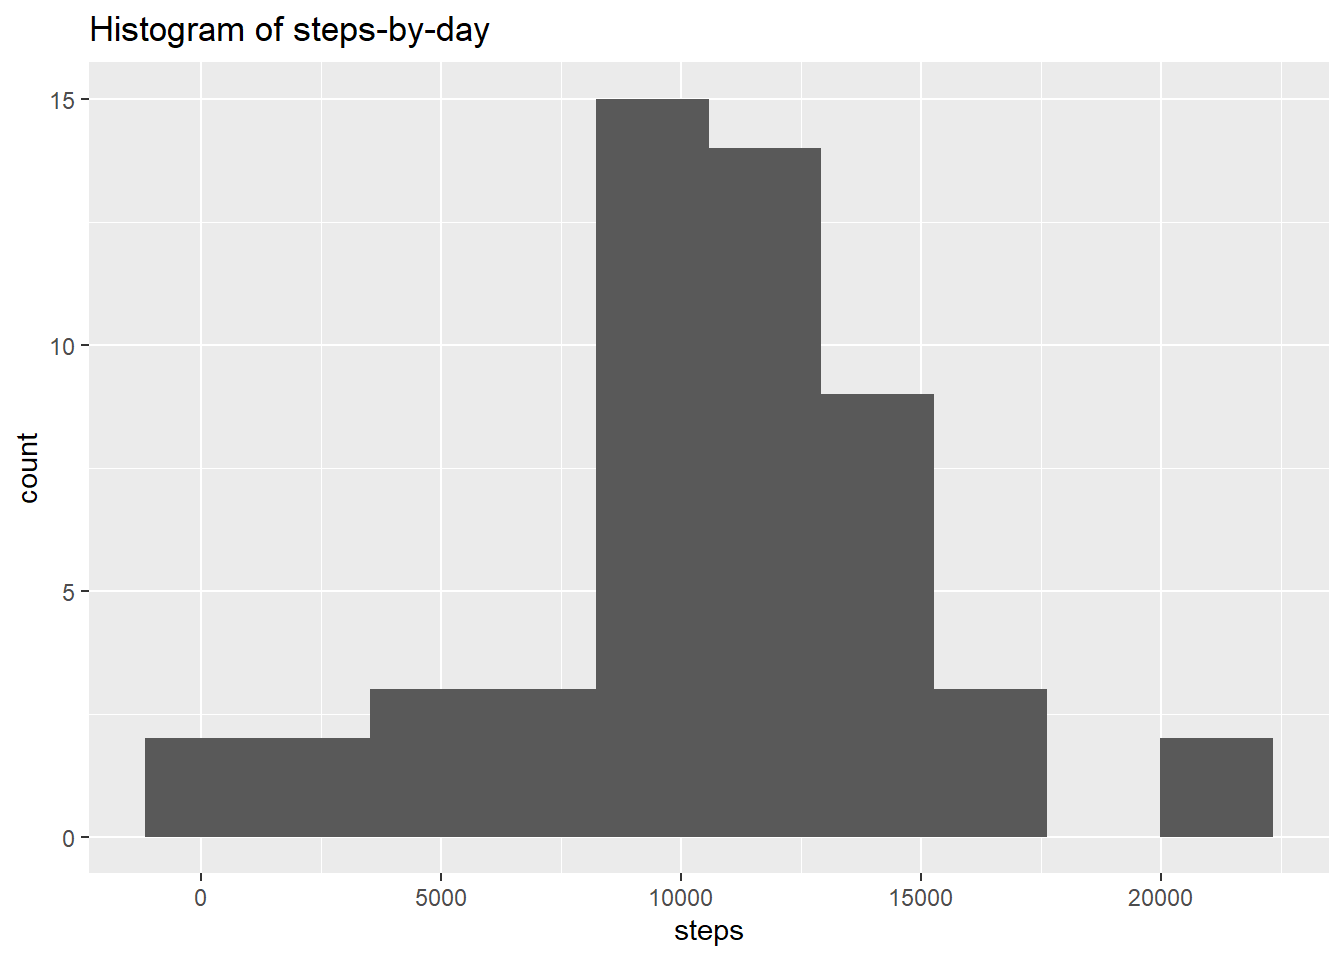
\includegraphics{PA1_template_files/figure-latex/Histogram_StepsByDay-1.pdf}
The general stats per day are:

\begin{Shaded}
\begin{Highlighting}[]
\FunctionTok{summary}\NormalTok{(df\_by\_day)}
\end{Highlighting}
\end{Shaded}

\begin{verbatim}
##       date                steps      
##  Min.   :2012-10-01   Min.   :   41  
##  1st Qu.:2012-10-16   1st Qu.: 8841  
##  Median :2012-10-31   Median :10765  
##  Mean   :2012-10-31   Mean   :10766  
##  3rd Qu.:2012-11-15   3rd Qu.:13294  
##  Max.   :2012-11-30   Max.   :21194  
##                       NA's   :8
\end{verbatim}

The \textbf{mean} number of steps was 10766 steps.\\
The \textbf{median} number of steps was 10765 steps.

\hypertarget{review-of-the-5-minute-interval-information}{%
\subsection{Review of the 5-minute interval
information}\label{review-of-the-5-minute-interval-information}}

\begin{Shaded}
\begin{Highlighting}[]
\NormalTok{df\_avg\_by\_day }\OtherTok{\textless{}{-}} \FunctionTok{aggregate}\NormalTok{(raw\_data}\SpecialCharTok{$}\NormalTok{steps, }\AttributeTok{by =} \FunctionTok{list}\NormalTok{(}\FunctionTok{ymd}\NormalTok{(raw\_data}\SpecialCharTok{$}\NormalTok{date)), }\AttributeTok{FUN =}\NormalTok{ mean)}
\NormalTok{df\_avg\_by\_day }\OtherTok{\textless{}{-}} \FunctionTok{setNames}\NormalTok{(df\_avg\_by\_day, }\FunctionTok{c}\NormalTok{(}\StringTok{"date"}\NormalTok{, }\StringTok{"mean\_steps"}\NormalTok{))}
\end{Highlighting}
\end{Shaded}

For the 5-minute range per day average

\begin{Shaded}
\begin{Highlighting}[]
\FunctionTok{ggplot}\NormalTok{(}\AttributeTok{data =}\NormalTok{ df\_avg\_by\_day, }\FunctionTok{aes}\NormalTok{(}\AttributeTok{x=}\NormalTok{date, }\AttributeTok{y=}\NormalTok{mean\_steps)) }\SpecialCharTok{+}
  \FunctionTok{geom\_line}\NormalTok{ () }\SpecialCharTok{+}
  \FunctionTok{labs}\NormalTok{(}\AttributeTok{title =} \StringTok{"Mean steps in the 5{-}minute range by day"}\NormalTok{)}
\end{Highlighting}
\end{Shaded}

\begin{verbatim}
## Warning: Removed 2 rows containing missing values (`geom_line()`).
\end{verbatim}

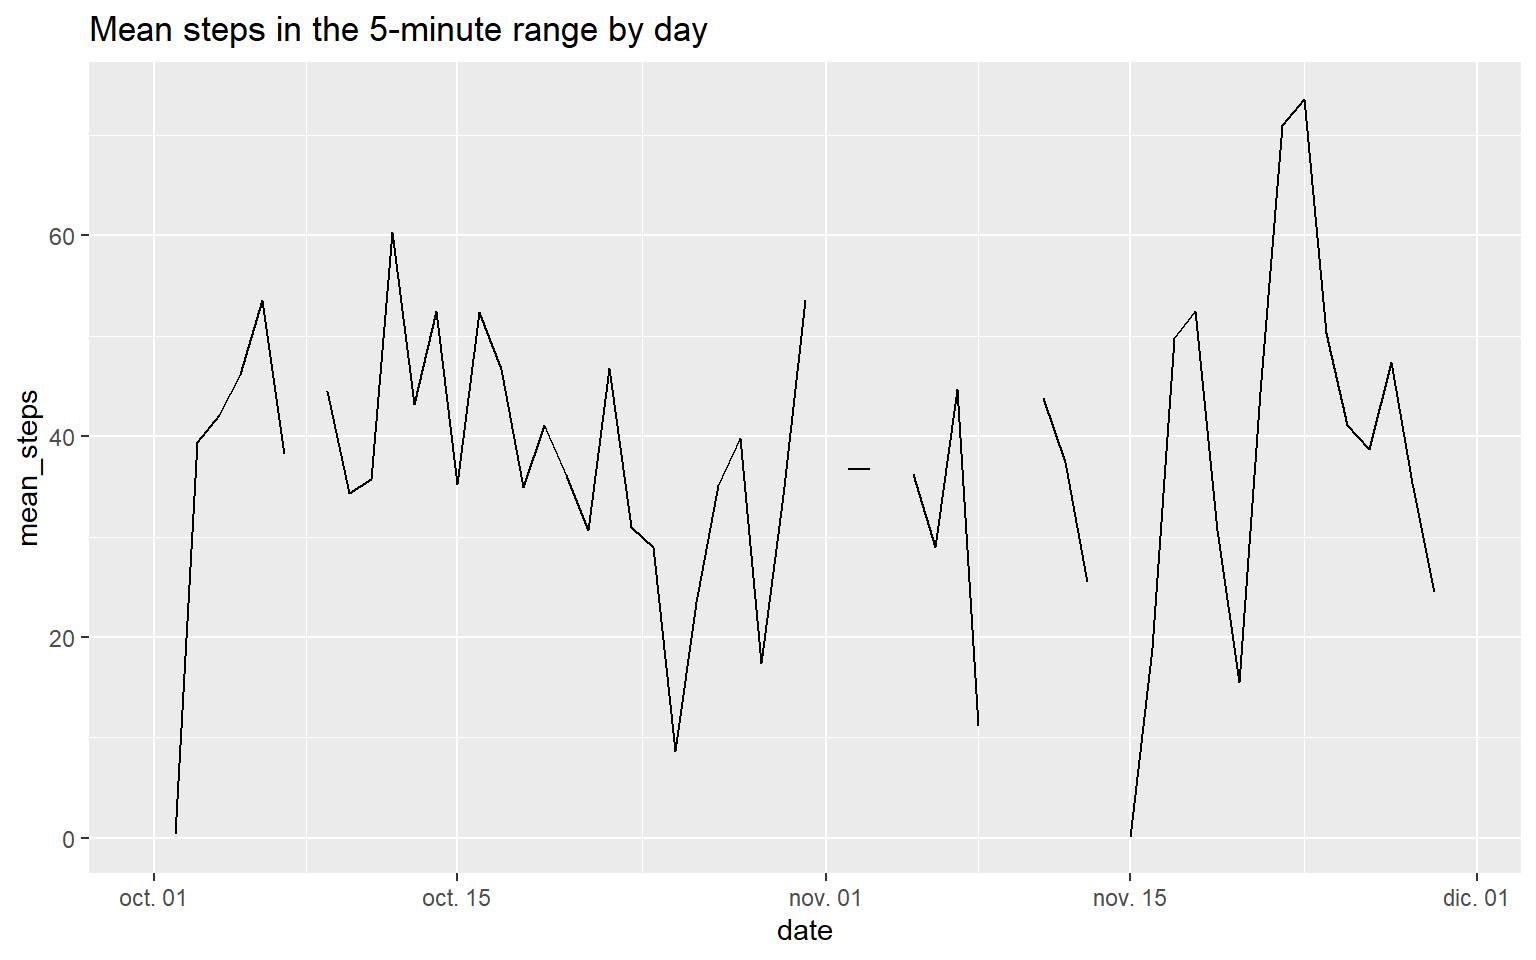
\includegraphics{PA1_template_files/figure-latex/line_plot-1.pdf} As it
is natural, there are 5-minute intervals with higher and lower activity
through the day.

The highest 5-minute intervals are around 8am with some peaks at 15hrs,
13hrs and 18hrs. The initial part of the day, before 5am, the number of
steps is near to zero, and after 19hrs it starts to decrease till the
end of the day. This activity registration makes sense of what could be
expected.

\begin{Shaded}
\begin{Highlighting}[]
\FunctionTok{ggplot}\NormalTok{(}\AttributeTok{data =}\NormalTok{ df\_avg\_by\_interval, }\FunctionTok{aes}\NormalTok{(}\AttributeTok{x=}\NormalTok{interval, }\AttributeTok{y=}\NormalTok{mean\_steps)) }\SpecialCharTok{+}
  \FunctionTok{geom\_line}\NormalTok{ () }\SpecialCharTok{+}
  \FunctionTok{labs}\NormalTok{(}\AttributeTok{title =} \StringTok{"Mean steps by the 5{-}minute intervals"}\NormalTok{)}
\end{Highlighting}
\end{Shaded}

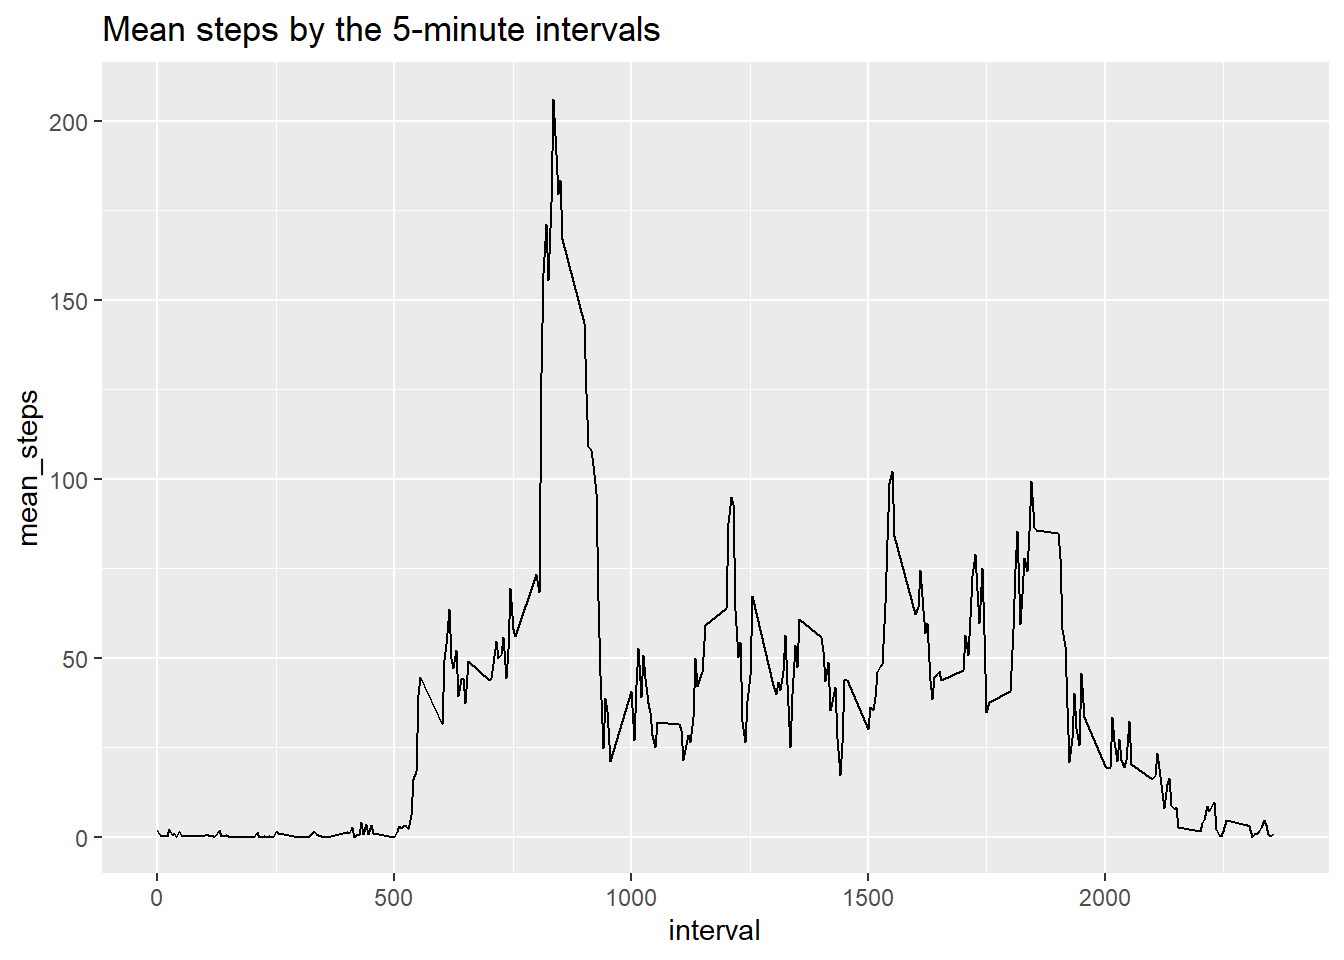
\includegraphics{PA1_template_files/figure-latex/line_plot_interval-1.pdf}
\#\#\# Filling NA's with average interval steps NA's values will be
filled with the average of each 5-minute interval will be added in order
to avoid impacting the overall average registered.

\begin{Shaded}
\begin{Highlighting}[]
\NormalTok{df\_filled\_na }\OtherTok{\textless{}{-}}\NormalTok{ raw\_data}

\ControlFlowTok{for}\NormalTok{ (i }\ControlFlowTok{in} \DecValTok{1}\SpecialCharTok{:}\FunctionTok{nrow}\NormalTok{(df\_avg\_by\_interval)) \{}
\NormalTok{  interval }\OtherTok{\textless{}{-}}\NormalTok{ df\_avg\_by\_interval}\SpecialCharTok{$}\NormalTok{interval[i]}
\NormalTok{  average\_value }\OtherTok{\textless{}{-}}\NormalTok{ df\_avg\_by\_interval}\SpecialCharTok{$}\NormalTok{mean\_steps[i]}
  
\NormalTok{  df\_filled\_na}\SpecialCharTok{$}\NormalTok{steps[}\FunctionTok{is.na}\NormalTok{(df\_filled\_na}\SpecialCharTok{$}\NormalTok{steps) }\SpecialCharTok{==} \ConstantTok{TRUE} 
                     \SpecialCharTok{\&}\NormalTok{ df\_filled\_na}\SpecialCharTok{$}\NormalTok{interval }\SpecialCharTok{==}\NormalTok{ interval] }\OtherTok{\textless{}{-}}\NormalTok{ average\_value}
  
\NormalTok{\}}
\end{Highlighting}
\end{Shaded}

\begin{Shaded}
\begin{Highlighting}[]
\NormalTok{df\_filled\_na\_by\_day }\OtherTok{\textless{}{-}} \FunctionTok{aggregate}\NormalTok{(df\_filled\_na}\SpecialCharTok{$}\NormalTok{steps, }\AttributeTok{by =} \FunctionTok{list}\NormalTok{(}\FunctionTok{ymd}\NormalTok{(df\_filled\_na}\SpecialCharTok{$}\NormalTok{date)), }\AttributeTok{FUN =}\NormalTok{ sum)}
\NormalTok{df\_filled\_na\_by\_day }\OtherTok{\textless{}{-}} \FunctionTok{setNames}\NormalTok{(df\_filled\_na\_by\_day, }\FunctionTok{c}\NormalTok{(}\StringTok{"date"}\NormalTok{, }\StringTok{"steps"}\NormalTok{))}
\end{Highlighting}
\end{Shaded}

\begin{Shaded}
\begin{Highlighting}[]
\FunctionTok{ggplot}\NormalTok{(}\AttributeTok{data =}\NormalTok{ df\_filled\_na\_by\_day, }\FunctionTok{aes}\NormalTok{(}\AttributeTok{x=}\NormalTok{date, }\AttributeTok{y=}\NormalTok{steps)) }\SpecialCharTok{+}
  \FunctionTok{geom\_bar}\NormalTok{(}\AttributeTok{stat=}\StringTok{"identity"}\NormalTok{) }\SpecialCharTok{+}
  \FunctionTok{labs}\NormalTok{(}\AttributeTok{title =} \StringTok{"Total steps by day"}\NormalTok{)}
\end{Highlighting}
\end{Shaded}

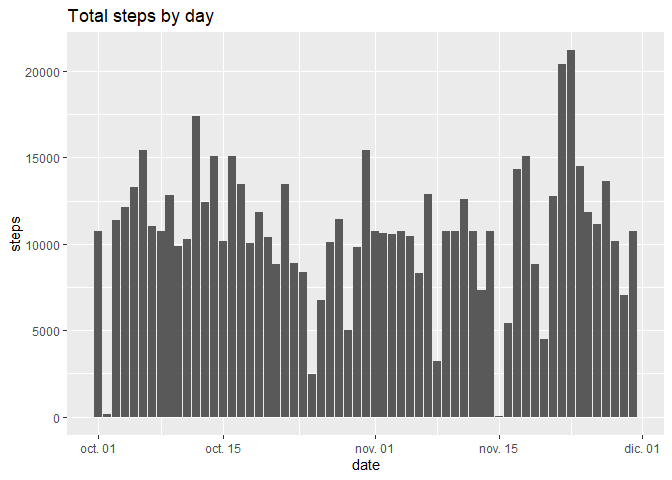
\includegraphics{PA1_template_files/figure-latex/Bar_StepsByDay_filledNA-1.pdf}

To make sure the filling of missing values did not affect the general
behavior previously reviewed, here are the General Stats and the
Histogram for the completed table.

\begin{Shaded}
\begin{Highlighting}[]
\FunctionTok{ggplot}\NormalTok{(}\AttributeTok{data =}\NormalTok{ df\_filled\_na\_by\_day, }\FunctionTok{aes}\NormalTok{(}\AttributeTok{x=}\NormalTok{steps)) }\SpecialCharTok{+}
  \FunctionTok{geom\_histogram}\NormalTok{(}\AttributeTok{bins =} \DecValTok{10}\NormalTok{) }\SpecialCharTok{+}
  \FunctionTok{labs}\NormalTok{(}\AttributeTok{title =} \StringTok{"Histogram of steps{-}by{-}day (filled NAs)"}\NormalTok{)}
\end{Highlighting}
\end{Shaded}

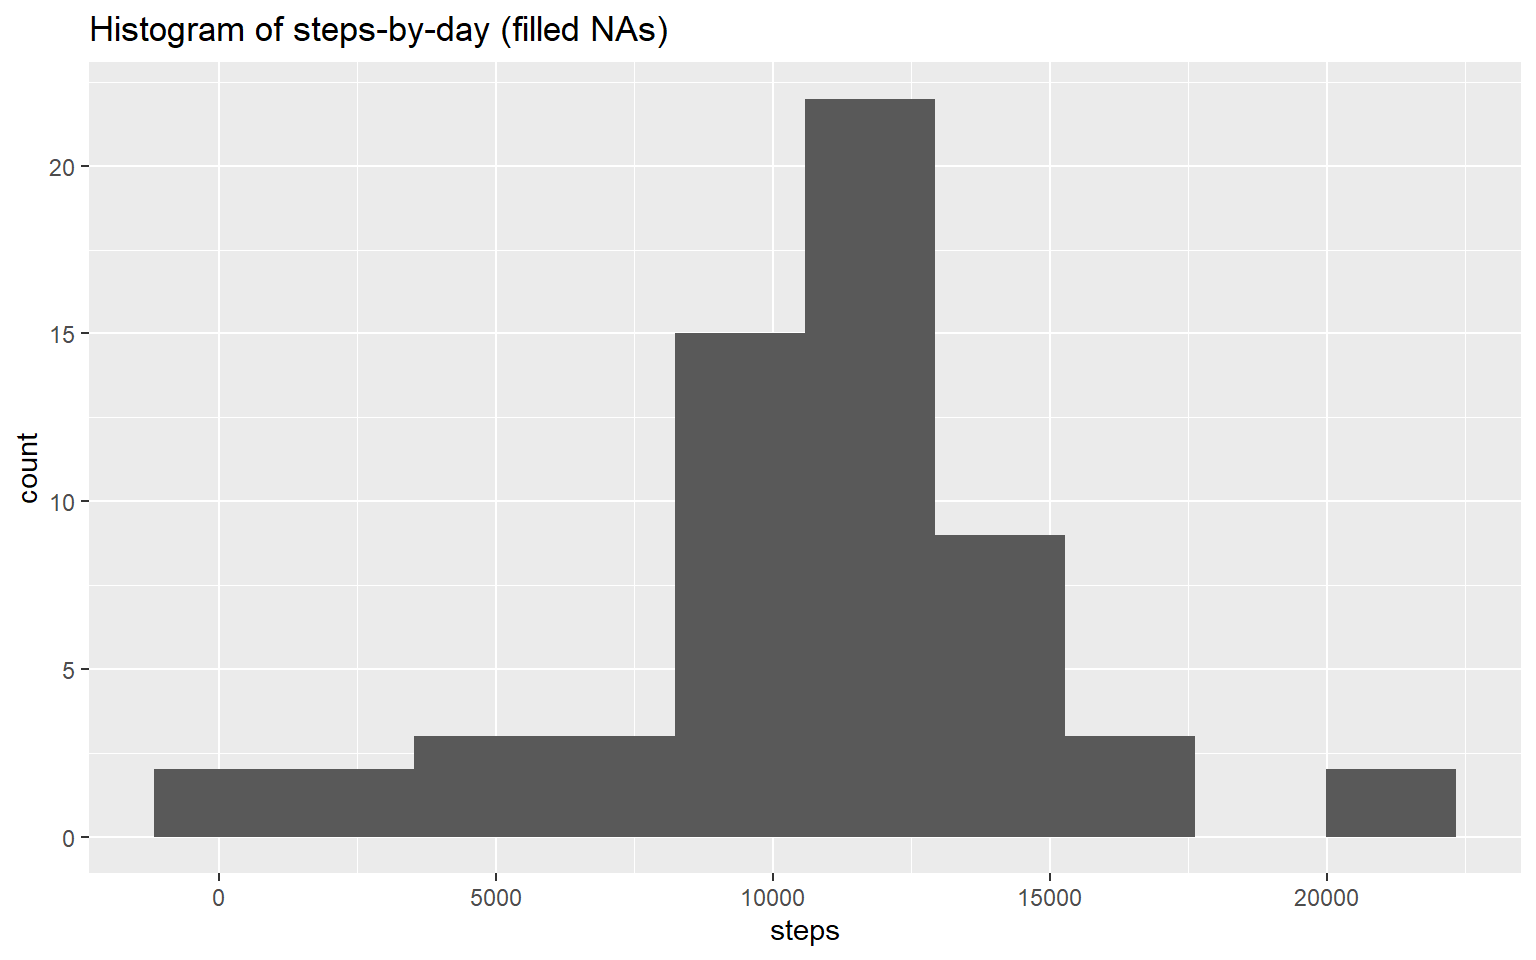
\includegraphics{PA1_template_files/figure-latex/Histogram_StepsByDay_filledNA-1.pdf}
The general stats per day are:

\begin{Shaded}
\begin{Highlighting}[]
\FunctionTok{summary}\NormalTok{(df\_filled\_na\_by\_day)}
\end{Highlighting}
\end{Shaded}

\begin{verbatim}
##       date                steps      
##  Min.   :2012-10-01   Min.   :   41  
##  1st Qu.:2012-10-16   1st Qu.: 9819  
##  Median :2012-10-31   Median :10766  
##  Mean   :2012-10-31   Mean   :10766  
##  3rd Qu.:2012-11-15   3rd Qu.:12811  
##  Max.   :2012-11-30   Max.   :21194
\end{verbatim}

The \textbf{mean} number of steps was 10766 steps.\\
The \textbf{median} number of steps was 10765 steps. The \textbf{mean}
and \textbf{median} remained almost equal, showing this method of
filling out missing values worked as expected.\\
And as it was expected, the 1st Quartile and 3rd Quartile did have some
change due to the add of values around in the mean range.

\hypertarget{weekdays-vs-weekends}{%
\subsubsection{Weekdays Vs Weekends}\label{weekdays-vs-weekends}}

During the weekdays it seems to be higher variance and the mean is
10177. For weekends, the mean is 12407.

\begin{Shaded}
\begin{Highlighting}[]
\FunctionTok{ggplot}\NormalTok{(}\AttributeTok{data =}\NormalTok{ df\_day\_type, }\FunctionTok{aes}\NormalTok{(}\AttributeTok{y=}\NormalTok{steps)) }\SpecialCharTok{+}
  \FunctionTok{geom\_boxplot}\NormalTok{() }\SpecialCharTok{+}
  \FunctionTok{facet\_wrap}\NormalTok{(}\SpecialCharTok{\textasciitilde{}}\NormalTok{Day) }\SpecialCharTok{+}
  \FunctionTok{labs}\NormalTok{(}\AttributeTok{title =} \StringTok{"Boxplot for Weekends Vs Weekdays"}\NormalTok{)}
\end{Highlighting}
\end{Shaded}

\begin{verbatim}
## Warning: Removed 8 rows containing non-finite values (`stat_boxplot()`).
\end{verbatim}

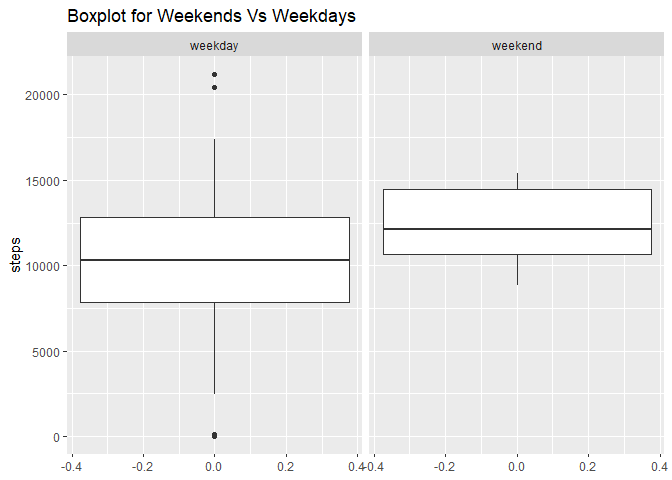
\includegraphics{PA1_template_files/figure-latex/Histogram_by_day_type-1.pdf}

\end{document}
